\chapter{Описание предлагаемого подхода для 3D локализации}

В этой главе будут описан предлагаемое решение задачи 3D локализации новообразований по снимкам КТ легких.

\section{Модель локализации опухолей}

Для детекции опухолей была заимстована сверточная сеть с архитектурой Squeeze and Excitation Encoder Decoder. Сеть использует архитектуру ResNet18 в качестве кодировщика со встроенными SE модулями после каждого сверточного блока ResNet (остаточного блока). 

\begin{figure}[!h]
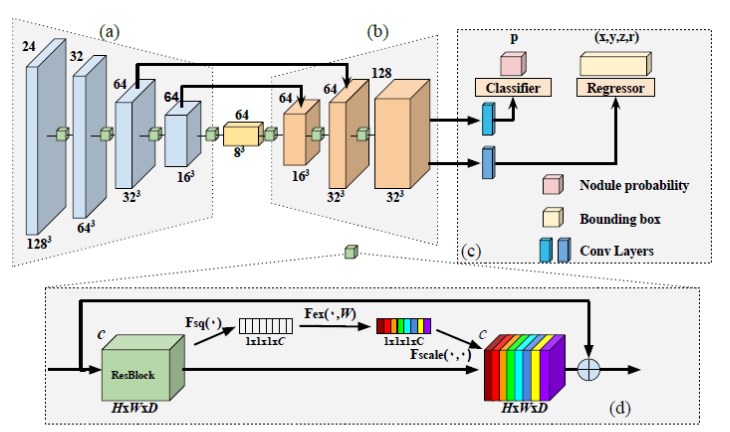
\includegraphics[width=\linewidth]{deep-seed-architecture.png}
\caption{Архитектура используемой сети DeepSEED}\label{deep-seed-architecture}
\centering
\end{figure}


\section{Аугментация данных с помощью генеративных противоборствующих сетей}

Широко известно применение генератиных противоборствующих сетей для генерации данных, которые впоследствии могут быть использованы в качестве расширения существующего датасета, на котором предполагается обучать детектор. В ряде работ были проведены визуальные тесты Тьюринга, где радиологам было предложено попробовать отличить генерированные опухоли от оригинальных. Специалисты не очень хорошо справились с задачей, что может говорить о том, что сети способны генерировать достаточно хорошие изображения, чтобы их можно было использовать в обучающем множестве.

\subsection{Модель генеративной противоборствующей сети}

Для решения данной задачи было принято решение заимствовать сеть, предложенную в работе []. У данной статьи есть документированная и удобная реализация в открытом доступе, в которой реализованы два фреймворка - один предназначен для добавления генерированных опухолей на изображение, второй предназначем для удаления опухолей с изображения. Для задачи аугментации данных естественно позаимствовать первый фреймворк который помимо реализации непосредственно архитектуры сети, предоставляет еще и возможность предобработки данных, которая состоит из нормализации и гистограммного выравнивания изображений.

Модель построена на условных GAN (Conditional GAN, CGAN), и основной задачей генератора является создание правдоподобной опухоли из некоторого шума и контекста. Сеть получает на вход $x_r^*$ - участок КТ изображения размера $32^3$, содержащий опухоль, из которого вырезан центральный куб размера $16^3$, и на его место вставлен некоторый случайный шум. Оставшаяся часть участка $x_r^*$ выступает в роли контекстного окружения. Сеть генератора состоит из нескольких сверточных слоев (кодировщика) и нескольких декодирующих слоев, которые соединены с кодирующими слоями попарно (skip connection). После каждого сверточного блока применяется батчевая нормализация. Выход генератора - $G(x_r^*, \theta_g)$ наряду с оригинальным участком изображения $x_r$ далее подаются на вход дискриминатору, задачей которого является классифицировать объекты как оригинальные или генерированные.

\begin{figure}[!h]
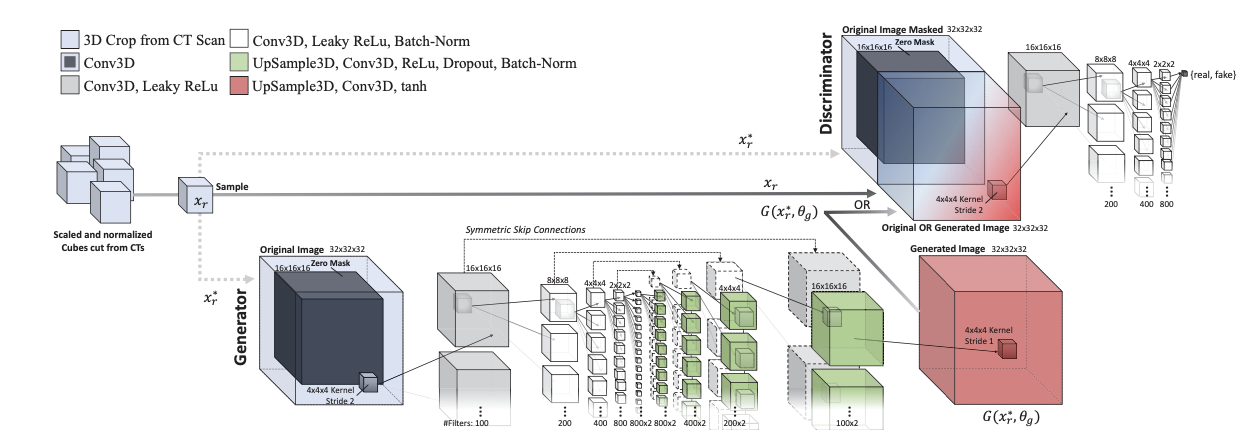
\includegraphics[width=\linewidth]{mirskiy-cgan-architecture.png}
\caption{Архитектура используемой сети CGAN}\label{mirskiy-cgan-architecture}
\centering
\end{figure}

\subsection{Адаптивная нормализация объектов (AdaIN)}

Адаптивная нормализация является популярной технологией и служит альтернативой батчевой нормализации и объектной нормализации, применяемой после каждого сверточного блока. Поэтому для совершенствования генеративной сети было предложено использовать ее вместо батчевой нормализации для эффективного и обучаемого преобразования промежуточных данных.

Адаптивная нормализация применяется следующим образом: $x$, являющийся входным тензором с размерностями (batchSize, xdim, ydim, zdim, channels) нормализуется по все пространственным измерениям, то есть это происходит независимо для каждого канала и объекта в отличие от батчевой нормализации и аналогично объектной нормализации (Instance Normalization). Параметры афинного преобразования имеют размерность (batchSize, 1, 1, 1, channels), то есть данные параметры аналогично варьируются по каналам и объектам.

\section{Итоговая модель обучения}

В результате предложенная модель обучения имеет следующий вид:

\begin{enumerate}
    \item Из датасета КТ изображений легких выбираются те, которые удовлетворяют некоторым ограничениям и соответственно являются пригодными для обучения CGAN
    \item Из выбранных данных вырезанются участки, содержащие опухоль, для создания объектов, которые можно непосредственно подать на вход CGAN.
    \item Данные аугментируются стандартными способами (повороты, отражения)
    \item Данные проходят предобработку: гистограммное выравнивание и нормализацию
    \item Данные, снабженные шумом на месте опухоли и окружающим контекстом подаются на вход CGAN для обучения
    \item Сеть CGAN, натренированная генерировать опухоли получает на вход предобработанные контексты для непосредственной генерации
    \item Данные, полученные на выходе CGAN, дополняют оригинальный датасет
    \item Сеть DeepSEED обучается на дополненном датасете.
\end{enumerate}

В следующую главу:

 В частности данный подход был реализован в [], где было предложено использовать Wassertstein GAN для аугментации датасета LIDC-IDRI

Важным является также тот момент, что эмпирически было установлено, что количество данных в обучающем множестве значительно влияет на качество модели, что опять-таки подтверждает предположение об уместности аугментации данных.

